\documentclass[reprint,english,notitlepage]{revtex4-2}  % defines the basic parameters of the document

% if you want a single-column, remove reprint

% allows special characters (including æøå)
\usepackage[utf8]{inputenc}
\usepackage[english]{babel}
\usepackage{float}
%% note that you may need to download some of these packages manually, it depends on your setup.
%% I recommend downloading TeXMaker, because it includes a large library of the most common packages.

\usepackage{physics,amssymb}  % mathematical symbols (physics imports amsmath)
\usepackage{graphicx}         % include graphics such as plots
\usepackage{xcolor}           % set colors
\usepackage{hyperref}         % automagic cross-referencing (this is GODLIKE)
\usepackage{tikz}             % draw figures manually
\usepackage{listings}         % display code
\usepackage{subfigure}        % imports a lot of cool and useful figure commands

% defines the color of hyperref objects
% Blending two colors:  blue!80!black  =  80% blue and 20% black
\hypersetup{ % this is just my personal choice, feel free to change things
    colorlinks,
    linkcolor={red!50!black},
    citecolor={blue!50!black},
    urlcolor={blue!80!black}}

%% Defines the style of the programming listing
%% This is actually my personal template, go ahead and change stuff if you want
\lstset{ %
	inputpath=,
	backgroundcolor=\color{white!88!black},
	basicstyle={\ttfamily\scriptsize},
	commentstyle=\color{magenta},
	language=Python,
	morekeywords={True,False},
	tabsize=4,
	stringstyle=\color{green!55!black},
	frame=single,
	keywordstyle=\color{blue},
	showstringspaces=false,
	columns=fullflexible,
	keepspaces=true}


%% USEFUL LINKS:
%%
%%   UiO LaTeX guides:        https://www.mn.uio.no/ifi/tjenester/it/hjelp/latex/ 
%%   mathematics:             https://en.wikibooks.org/wiki/LaTeX/Mathematics

%%   PHYSICS !                https://mirror.hmc.edu/ctan/macros/latex/contrib/physics/physics.pdf

%%   the basics of Tikz:       https://en.wikibooks.org/wiki/LaTeX/PGF/TikZ
%%   all the colors!:          https://en.wikibooks.org/wiki/LaTeX/Colors
%%   how to draw tables:       https://en.wikibooks.org/wiki/LaTeX/Tables
%%   code listing styles:      https://en.wikibooks.org/wiki/LaTeX/Source_Code_Listings
%%   \includegraphics          https://en.wikibooks.org/wiki/LaTeX/Importing_Graphics
%%   learn more about figures  https://en.wikibooks.org/wiki/LaTeX/Floats,_Figures_and_Captions
%%   automagic bibliography:   https://en.wikibooks.org/wiki/LaTeX/Bibliography_Management  (this one is kinda difficult the first time)
%%   REVTeX Guide:             http://www.physics.csbsju.edu/370/papers/Journal_Style_Manuals/auguide4-1.pdf
%%
%%   (this document is of class "revtex4-1", the REVTeX Guide explains how the class works)


%% CREATING THE .pdf FILE USING LINUX IN THE TERMINAL
%% 
%% [terminal]$ pdflatex template.tex
%%
%% Run the command twice, always.
%% If you want to use \footnote, you need to run these commands (IN THIS SPECIFIC ORDER)
%% 
%% [terminal]$ pdflatex template.tex
%% [terminal]$ bibtex template
%% [terminal]$ pdflatex template.tex
%% [terminal]$ pdflatex template.tex
%%
%% Don't ask me why, I don't know.

\begin{document}
\title{This is a Very Important Title!}   % self-explanatory
\author{Person McSomething}               % self-explanatory
\date{\today}                             % self-explanatory
\noaffiliation                            % ignore this
\begin{abstract}                          % marks the beginning of the abstract
This abstract is abstract.                % the body of the abstract
\end{abstract}                            % marks the end of the abstract
\maketitle                                % creates the title, author, date & abstract

If you want to learn more about using \LaTeX, you should check UiO's official tutorials:
\url{https://www.mn.uio.no/ifi/tjenester/it/hjelp/latex/}

If you are familiar with \LaTeX\ and you want to learn more about the REVTeX4-1 document class, check:
\url{http://www.physics.csbsju.edu/370/papers/Journal_Style_Manuals/auguide4-1.pdf}


% the fundamental components of scientific reports:
\section{Introdukson}

\section{Mal jeg må endre på}
Vi starter med et $2\cross 2$ gitter og skal regne dette analytisk slik at vi kan gjøre en sammenlikning med vårt numeriske resultat. Vi ser at hver kombinasjon av ett spinn opp vil være en rotert versjon av de andre kombinasjonene av ett spinn opp. Den samme rotasjonsegenskapen ser vi med tre spinn opp, siden det også bare er ett spinn ned. Med to spinn opp derimot, ser vi at vi får flere kombinasjoner. Vi har igjen fire roterte versjoner hvor spinn opp-partiklene er ved siden av hverandre, men også to hvor de er diagonale til hverandre.
For å finne energien vil vi trenge
$$
E(s)=-J\sum_{<kl>}^N s_k \cdot s_l
$$
Hvor $<kl>$ betyr at vi går over alle partiklene uten å telle interaksjonen mellom partiklene to ganger. $s_l$ og $s_k$ vil også være nabopartikler i gitteret. Vi vil i alle forsøkene, også utenfor $2\cross 2$ eksempelet anta periodiske grensebetingelser. Det vil si at vi antar at i hver ende vil nabopartikelen være den motsatte enden. Man kan tenke seg at i én dimensjon så vil partiklene være i en sirkel hvor endene møtes.
\newline 
Vi skal også regne det magnetiske feltet gitt ved
$$
M(\mathbf{s})=\sum_i s_i
$$
\section{Teori}
Vi skal regne for tilstander $\mathbf{s}$ gitt som et 2D $L\cross L$ gitter med partikler $s_i$ som enten kan ha tilstanden spinn opp eller spinn ned. Vi setter at dersom $s_i$ har tilstanden spinn opp så er $s_i=+1$ og hvis $s_i$ har spinn ned er $s_i=-1$. Vi vil bruke periodiske grensebetingelser slik at naboen til $s_1$ som er lengst til venstre vil har $s_L$ som er lengst til høyre som sin venstre nabo. Det samme gjelder da lodrett, så den øverste spinnet vil ha den nederste parikkelen som sin nabo. I dette forsøket antar vi at ved å bruke Hamiltonianeren på en slik state gir energien
$$
E(\mathbf{s})=-J\sum_{\expval{kl}}^{N} s_k s_l
$$
hvor $\expval{kl}$ betyr at den går gjennom det energien mellom hvert spinn og deres naboer én gang og teller ikke dette to ganger. $J$ vil være koblingskonstant. $N=L^2$ altså størrelsen av $\mathbf{s}$ slik at vi går gjennom hele matrisen.
\newline Vi har også energien per spin $\epsilon$ gitt ved 
$$
\epsilon(\mathbf{s}) =\frac{E(\mathbf{s})}{N}
$$
som vi må bruke når vi skal sammenligne matriser av ulike størrelser.
\newline Vi trenger også magnetisaseringen gitt ved
$$
M(\mathbf{s})=\sum_i^N s_i
$$
så vi da får en magnetisasjon per spin som
$$
m(\mathbf{s})=\frac{\mathbf{s}}{N}
$$
Vi skal også finne forventingsverdiene $\expval{\epsilon}$ og $\expval{|m|}$. Forventingsverdien i dette systemet er gitt ved
$$
\expval{a}=\sum _i^{N}a(\mathbf{s}_i) p(\mathbf{s}_i)
$$
hvor vi her går gjennom alle mulige tilstander $\mathbf{s}_i$ som systemet av denne størrelsen kan være i. $Z$ er her partisjonsfunksjonen gitt som
$$
Z=\sum_{i}^{N}e^{\beta \mathbf{s_i}}
$$
hvor $\beta=\frac{1}{k_bT}$. \newline  Vi skal også finne den spesifike varmekapasiteten
$$
C_V=\frac{1}{k_B T^2}(\expval{\epsilon}^2-\expval{\epsilon}^2)
$$
og den susceptilbiliteten
$$
\chi =\frac{1}{k_B T}(\expval{m^2}-\expval{m}^2-\expval{|m|}^2)
$$
så vi må også finne $\expval{\epsilon^2}$ og $\expval{m^2}$. \newline
Når vi flipper et spinn så skal vi også kunne få en energiendring gitt ved
$$
\Delta E=E(\mathbf{s}_{etter})-E(\mathbf{s}_{før})=E_(\mathbf{s}_a)-E(\mathbf{s}_b)
$$
Utvider vi det får vi
$$
\Delta E=-J\sum_{\expval{kl}}^{N} s_{a_k} s_{l_a}-(-J)\sum_{\expval{kl}}^{N} s_{k_b} s_{l_b}
$$
$$
\Delta E=-J\sum_{\expval{kl}}^{N} s_{k_a}s_{l_a}-s_{k_b}s_{l_b}
$$
La oss si at vi flipper spinnet $s_{i,j}$ hvor $i$ representerer den vannrette posisjonen og $j$ den lodrette. Da kun $s_{k_b}s{l_b}$ kun endre seg hvor $s_{i,j}$ er en av faktorene. Ellers vil $s_{k_b}s_{l_b}=s_{k_a}s_{l_a}$ og her vil $s_{k_a}s_{l_a}-s_{k_b}s_{l_b}=0$. Vi står da kun igjen med
$$
\Delta E= -J \begin{pmatrix} s_{i,j-1}s_{i,j_a}-s_{i,j-1}s_{i,j_b}+s_{i+1,j}s_{i,j_a}-s_{i+1,j}s_{i,j_b} \\+ s_{i,j+1}s_{i,j_a}-s_{i,j+1}s_{i,j_b}+s_{i-1,j}s_{i,j_a}-s_{i-1,j}s_{i,j_b}\end{pmatrix}
$$
Vi kan så ta ut $(s_{i,j_a}-s_{i,j_b}$ og få
$$
\Delta E=-J(s_{i,j_a}-s_{i,j_b})(
s_{i.j-1}+s_{i+1,j} +s_{i,j+1}+s_{i-1.j}
)
$$
Vi ser at $s_{i,j_a}-s_{i,j_b}$ er enten $+1-(-1)=2$ når den skifter fra spin ned til opp og $-1-(+1)=-2$ når den skifter fra spin opp til ned. Ellers må vi også naboleddene somhar fem muligheter
$$
1+1+1+1=4
$$
$$
1+1+1-1=2
$$
$$
1+1-1-1=0
$$
$$
1-1-1-1=-2
$$
$$
-1-1-1-1=-4
$$
Så vi får altså 5 mulige forskjeller i energi

\section{Metode}
\section{Resultater}
\section{Diskusjon}
\section{Conklusjon}
% acknowledgements (optional)
\begin{acknowledgments}  % if you disagree with the spelling, blame Americans
I would like thank myself for writing this beautiful document.
\end{acknowledgments}


%% When it comes to the bibliography I personally generate it using BibLaTeX. (see the link above if you're interested)
%% You're obviously allowed to create the references section however you like.
%% I'll keep it simple here.
\section*{References}  % the asterisk (*) after \section makes the section numbering go away
\begin{itemize}
\item[-]Reference 1
\item[-]Reference 2
\end{itemize}

\newpage
%% if you want to include an appendix, this is how you do it
\appendix
\section{$2\cross 2$ gitter}
Vi starter med å finne alle mulige tilstander for et $2\cross 2$ gitter, som gitt i figur \ref{2x2}
\begin{figure}[H]
	\label{2x2}
	\includegraphics[scale=0.5]{Latice.pdf}
	\caption{Alle tilstander som er mulig i et $2\cross2$-gitter. En rute med en prikk i seg betyr at dette spinnet har spin opp altså $+1$, mens en blank rute betyr at dette spinnet har spin ned, altså $-1$}
\end{figure}
Vi ser altså at det er 16 forskjellige muligheter tilstander i et $2\cross2$-gitter, men noen av disse er symmetriske. Alle fire tilstandene med ett spin opp er symmetriske, det samme gjelder for ett spin ned. Alle tilstandene for to spin opp hvor to av dem er naboer er har også en symmetri og det samme med de to diagonale. Vi kan derfor si at de som er symmetriske har samme total energi og da trenger vi bare å finne en av disse som er symmetriske til hverandre for å finne alle. Da blir disse tilstandene også energidegenererte. Vi får da en tabell gitt som i \ref{2x2tabell}
\begin{table}[H]
	\begin{tabular}{|c|c|c|c|} % note that & separates columns while \\ separates the rows
		\hline                    % creates a horizontal line (try removing it)
		Antall spin opp & $E(s)$ & $M(s)$& Degenerasjon  \\
		\hline
		$0$ & $-8J$ & $-4$ & $4$ \\
		\hline
		$1$ & $0$ & $-2$ & 4\\
		\hline
		$2$ &$0$ &$0$ &$4$ \\\hline 
		$2$ &$8J$ &$0$&$2$ \\\hline 
		$3$&$0$&$2$&$4$ \\\hline 
		$4$&$-8J$&$4$&$1$ \\\hline 
	\end{tabular}
\caption{En tabell med verdiene til $2\cross 2$ matrisen}
\label{2x2tabell}
\end{table}
Så kan vi bruke dette til å finne den andre verdiene. Først ser vi på $Z$, som blir 
$$
Z=\sum_s=e^{-\beta E(s)}=12 e^{0}+2e^{-\beta (-8J)}+2e^{-\beta 8J}=12+4\cosh(8\beta)
$$
Så finner vi $\expval{\epsilon}$, altså
$$
\expval{\epsilon}=\sum_{s}p(s)\frac{E(s)}{N}=\sum_{s}\frac{e^{-\beta E(s)}E(s)}{N}
$$
$$
\expval{\epsilon}=\frac{-8Je^{8J}\cdot 2 + 8Je^{-\beta 8J}\cdot 2}{NZ}=\frac{-16J}{NZ}(e^{8\beta J}-e^{-8\beta J})$$$$\expval{\epsilon}=-\frac{-16 J}{4Z}2\sinh(8\beta J)=\frac{-8J}{Z}\sinh(8J\beta)
$$
Så finner vi $\expval{\epsilon^2}$ med 
$$
\expval{\epsilon^2}=\sum_{s}\frac{E(s)^2}{N^2}p(s)=\sum_{s}e^{-\beta E(s)}\frac{E(s)^2}{N^2Z}
$$
$$
\expval{\epsilon^2}=\frac{2(8J)^2e^{8J\beta}+2(8J)^2e^{-8J\beta}}{N^2Z}=\frac{2(8J)^2}{N^2Z}\cosh(8J\beta)
$$
$$
\expval{\epsilon^2}=4(\frac{8J}{4})^2\cosh(8J\beta)=\frac{16J^2}{Z}\cosh(8J\beta)
$$
Så kan vi bruke disse til å finne
$$
C_V=\frac{1}{Nk_BT^2}(\expval{E^2}-\expval{E}^2)
$$
Hvor 
$$\expval{E}^2=(\expval{\epsilon\cdot N})^2=\expval{\epsilon}\cdot N)^2=(\frac{-8J\cdot 4}{Z}\sinh(8J\beta))^2$$så $$\expval{E}^2=(\frac{32J}{Z})^2\sinh^2(8J\beta)
$$
Mens
$$
\expval{E^2}=\expval{(\epsilon^2\cdot N^2)}=\frac{16^2J^2}{Z}\cosh(0J\beta)
$$
så vi får at
$$
C_V=\frac{1}{Nk_BT^2}(\frac{16^2J^2}{Z}\cosh(0J\beta)-(\frac{32J}{Z})^2\sinh^2(8J\beta))
$$
Så finner vi magnetiseringen
$$
\expval{|M|}=\sum_s |M(s)|p(s)=\frac{4e^{8J}+2e^0 +2e^0 +4e^{8J}}{Z}=4\frac{1+2e^{8J}}{Z}
$$
så 
$$
\expval{|m|}=\expval{\frac{|M|}{N}}=\frac{4}{4}\frac{1+2e^{8J\beta}}{Z}=\frac{1+2e^{8J\beta}}{Z}
$$
Så har vi
$$
\expval{M^2}=\sum_s M(s)^2p(s)=\frac{16e^{8J\beta+4+4+16e^{8J\beta}}}{Z}=8\frac{1+2e^{8J\beta}}{Z}
$$
så
$$
\expval{m^2}=\frac{8}{16}\frac{1+2e^{8J\beta}}{Z}=\frac{1+2e^{8J\beta}}{2Z}
$$
Da får vi at
$$
\chi 
$$
\section{This is another appendix}\label{appendix}
Tada.
%% all \section commands following \appendix are automatically taken as appendices

%% Note that \label{appendix} command on line 115. What this does is setup a reference point for LaTeX that you can
%% access wherever you want using \ref{appendix}.
%% You can place labels on most environments such as equations, figures, tables, etc.

\clearpage
Note that this document is written in the two-column format. If you want to display a large equation, a large figure, or whatever, in one-column format, you can do this like so:
\onecolumngrid
\vspace{1cm} % some extra space
This text and this equation are both in one-column format.

\footnote{This equation is actually from quantum mechanics. ``It's called Schrödinger's Time-Dependent Wave Equation'', named after the awesome Austrian physicist Erwin Rudolf Josef Alexander Schrödinger. Yep, the ``Schrödinger's cat'' guy. Pretty cool dude actually, check his wiki page: \url{https://en.wikipedia.org/wiki/Erwin_Schrodinger}. He was physics' no. 1 Ladies' man if there ever was one. Anyway, you will learn more about this equation in FYS2140. You can also find it printed on a glass wall in the UiO Physics Building (it really is that important).}

\begin{equation}\label{equation}
\frac{-\hbar^2}{2m}\laplacian{\Psi}+V\Psi=i\hbar\pdv{t}\Psi
\end{equation}
Note that the equation numbering (this: \ref{equation}) follows the appendix as this text is technically inside Appendix \ref{appendix}. If you want a detailed listing of (almost) every available math command, check: \url{https://en.wikibooks.org/wiki/LaTeX/Mathematics}.
\vspace{1cm} % some extra space
\twocolumngrid
And now we're back to two-column format. It's really easy to switch between the two. It's recommended to keep the two-column format, because it is easier to read, it's not very cluttered, etc. Pro Tip: You should also get used to working with REVTeX because it is really helpful in FYS2150.

One last thing, this is a code listing:
\begin{lstlisting}
This will be displayed with a cool programming font!
\end{lstlisting}
You can add extra arguments using optional parameters:
\begin{lstlisting}[morekeywords={cool}]
This will be displayed with a cool programming font!
\end{lstlisting}
You can also list code from a file using \texttt{lstinputlisting}. If you're interested, check \url{https://en.wikibooks.org/wiki/LaTeX/Source_Code_Listings}.

This is a basic table:
\begin{table}[h]  % h = "here"  , h! = here!
\caption{This is a nice table}\label{table}
\begin{tabular}{|c|c|c|} % note that & separates columns while \\ separates the rows
\hline                    % creates a horizontal line (try removing it)
Hey & Hey & Hey  \\
\hline
Hello & Hello & Hello \\
\hline
Bye & Bye & Bye \\
\hline
\end{tabular}
\end{table}\\
You can a detailed description of tables here: \url{https://en.wikibooks.org/wiki/LaTeX/Tables}.

I'm not going to delve into Tikz in any level detail, but here's a quick picture:
\begin{figure}[h]
\centering  % places the tikz image in the center of the text column
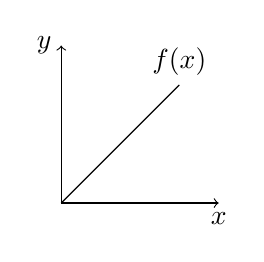
\begin{tikzpicture}
\draw[->] (0,0) -- (2,0) node [pos=1.0,below] {\(x\)};
\draw[->] (0,0) -- (0,2) node [pos=1.0,left] {\(y\)};
\draw (0,0) -- (1.5,1.5) node [pos=1.0,above] {\(f(x)\)};
\end{tikzpicture}
\caption{This is great caption}\label{figure}
\end{figure}\\
If you want to know more, check: \url{https://en.wikibooks.org/wiki/LaTeX/PGF/TikZ}.

%% If you want to include figure:
%\includegraphics[scale=1.0]{filename}
%% check https://en.wikibooks.org/wiki/LaTeX/Importing_Graphics if you want to know more

\end{document}
